\documentclass[12pt, letterpaper]{article}
\usepackage[top=1in, bottom=1in, left=1.5in, right=1.5in]{geometry}
\usepackage{amsmath}
\usepackage{amsfonts}
\usepackage{natbib}
\usepackage{mathtools}
\usepackage{amssymb}
\usepackage{fullpage}
\usepackage{listings}
\usepackage{float}
\usepackage{natbib}
\usepackage{url}
\usepackage[clockwise]{rotating}
\usepackage{caption}
\usepackage{graphicx}
\let\oldtabular\tabular
\renewcommand{\tabular}{\footnotesize\oldtabular}
%\newcommand\Fontvi{\fontsize{8}{7.2}\selectfont}

\lstset{language=R}
%\setlength{\textwidth}{150mm}
\linespread{1.6}
\bibpunct{(}{)}{;}{a}{,}{,}

\begin{document}
\title{Earnings Forecasts from Firm-Level Regressions: Implications for Research and Practice}
\author{Reginald Edwards\footnote{Ross School of Business, University of 
Michigan (\texttt{reggie@umich.edu}).}}
\date{This Draft: 1 September 2014}
\maketitle

\begin{abstract} 

%Short motivation. Short research question. Short contribution. Short conclusion.
Analyst 
forecasts are used in research  on valuation, cost of capital, and more. In this paper I deconstruct
this supposed advantage of analysts over statistical forecasts. I develop and evaluate a novel
statistical forecasting framework for earnings. I reinterpret and reevaluate estimates of firms' 
implied cost of capital and market-level risk premia that rely on analyst forecasts by using a 
statistical forecast. I examine if the main strength of the purported superioty of analyst forecasts
is concentrated in the period prior to the passage of Regulation Fair Disclosure (Reg FD). 
My work posits a model of earnings that has many of the 
desirable properties of analyst forecasts, but less bias and is applicable to more firms and years.
This model is thus more useful to both researchers and practitioners.

\end{abstract}

\section{Introduction}
The maintained assumption in accounting research is that analyst forecasts of firms' earnings are 
superior to forecasts from statistical models and represent a more accurate proxy for the market's
expectations of future corporate earnings. Thus, analyst 
forecasts are used in research  on valuation, cost of capital, and more. In this paper I deconstruct
this supposed advantage of analysts over statistical forecasts. I develop and evaluate a novel
statistical forecasting framework for earnings. I reinterpret and reevaluate estimates of firms' 
implied cost of capital and market-level risk premia that rely on analyst forecasts by using a 
statistical forecast. I examine if the main strength of the purported superioty of analyst forecasts
is concentrated in the period prior to the passage of Regulation Fair Disclosure (Reg FD). And, 
lastly, I evaluate a trading strategy that hinges on disagreement between the statistical forecast 
of earnings and analysts' expectations.
 
My work here is largely descriptive (and proscriptive) in nature and has a methodological purpose. 
The use of analyst forecasts of earnings as proxies for the market's expectations of earnings has 
been questioned in recent years. My work posits a model of earnings that has many of the 
desirable properties of analyst forecasts, but less bias and is applicable to more firms and years.
This model is thus more useful to both researchers and practitioners.
 
The accounting literature stands in contrast to many fields of economics and finance in the 
preeminence of expert judgment (that of equity research analysts) over statistical forecasts in the
realm of corporate earnings. Researchers and practitioners often use statistical forecasts to
augment or obviate professional, human forecasts of inflation (\cite{Faust20132}), GDP 
(\cite{Chauvet2013141}), interest rates (\cite{Duffee2013385}), oil prices 
(\cite{Alquist2013427}), and 
real estate prices (\cite{Ghysels2013509}). Indeed, these forecasts are often found to be superior
to human forecasts on various measures of performance evaluation and better proxies for market
expectations.

%<re-phrase>
Research that relies on analyst forecasts of earnings suffers from three flaws: (1) analyst 
forecasts are known to be upwardly biased; (2) there is evidence suggesting analysts don't
attempt to accurately forecast earnings and investors don't necessarily rely on these forecasts
explicitly for information about long-term cash flows; and (3) since the availability of machine-
readable analyst forecasts only dates back to the early 1980s, the research sample is necessarily
limited. The statistical forecasts of earnings from firm-level regressions that I develop here
overcomes the first and last points. By demonstrating that the forecasts from my model are 
associated with higher returns I provide support for the notion that some market participants
may be able to derive more accurate from the past history of earnings than is given by blindly
following analyst forecasts. To fully address the second point, the forecasts from my model must
be used to derive implied cost of capital estimates and market risk premia. 
%</re-phrase>

My work here contributes to the literature in two ways. The first is methodological in nature. I 
deconstruct the notion that analysts forecasts are the best estimates of earnings, develop a 
superior statistical framework for forecasting earnings, and discuss the implications for resarch 
design for using the analyst forecasts instead of the statistical forecasts. The second contribution
is more applied. I show how using a statistical forecast of earnings can be used to gain an edge
over market participants that rely on analyst forecasts.

\section{Literature Review}

\subsection{Statistical Earnings Forecasts}
Research on understanding and forecasting the time-series properties of earnings can be traced back
to at least the 1960s (\cite{little1962}). The earliest studies in accounting [e.g., 
\cite{ballwatts1972}, \cite{brooksbuckmaster1976}] concluded that earnings follow a random-walk
process and little could be gained from statistical 
earnings forecasts. Later, \cite{brown1993} lays out a coherent path for future research into 
earnings forecasts. A decade later, \cite{kothari2001} declares that this literature was ``fast 
becoming extinct'' due to the ready availability of analyst forecasts. However, 
\cite{bradshawetal2012} 
contribute to a recent resurgence in focus on the forecastability of earnings and the usefulness and
appropriateness of such forecasts to researchers and practitioners.

\cite{houvandijkzhang2012} represent an important step towards more sophisticated models of
earnings based on economically sound predictor variables. In the spirit of \cite{famafrench2000}, 
they develop a cross-sectional regression-based forecast of earnings. My work
here builds on and differs from theirs in key ways. The most prominent difference is in estimation
methodology and forecaste evaluation. \cite{houvandijkzhang2012} estimate their pooled regression 
over all firms for one year at a time. They then average the in-sample coefficients and use the
averaged coefficients to forecast earnings one to five years ahead. \cite{houvandijkzhang2012} also
use GAAP earnings (from Compustat) as opposed to ``street'' earnings-per-share (from IBES) to build
their model, thus making it difficult to compare the forecast accuracy of their model with that of
analysts.

\subsection{Analysts' Earnings Forecasts}
Analysts are generally seen to have two advantages over statistical models with respect to 
forecasting earnings: (1) analaysts have access to more recent data (the \emph{timing advantage},
and (2) analysts have access to proprietary information stemming from their access to management,
customers, and suppliers (the \emph{information advantage}.) With respect to the information 
advantage analysts are said to posses, it is likely that this would
deteriorate subsequent to the passage of Regulation Fair Disclosure (Reg. FD.) Reg. FD was designed to 
prohibit select groups of investors and analysts from gaining access to exclusive information from
management. Indeed, \cite{gintschelmarkov2004} find that analyst forecasts are less informative
after the passage of Reg. FD. Thus, findings of analyst superiority over time-series models are 
likely to attenuate over time.

Moreover, analyst forecasts tend to
exhibit well-documented and predictable biases. Empirical evidence suggests that analysts issue more
optimistic (upwardly biased) forecasts when (1) issuing buy recommendations [\cite{eamesetal2002}],
(2) forecasting lower earnings [\cite{francisphilbrick1993}], and (3) when the target firm's 
earnings are less predictable [\cite{dasetal1998}]. It is also unclear whether and to what extent investors
as a whole rely on analyst forecasts to form expectations about future earnings and, thus, price.
Given these considerations, it is natural to consider if statistical models of earnings that 
replicate much of the decision process undertaken by individual analysts can improve upon analyst
forecasts.

\subsection{Implications for Implied Cost of Capital Estimates}

An expectation of a firm's future earnings is the key input into estimates of that firm's cost of
capital as implied by its prevailing market price (\cite{gebhardtetal2001}). Reverse-engineering 
the cost of capital is essential for internal capital budgeting and external investment evaluation.
Also, aggregates of firm-level cost of capital estimates have been shown to have risk-return 
characteristics that more closely follow standard asset pricing theory (\cite{leeetal2011}). 
Standard in the literature is the use of analyst forecasts of earnings and long-term growth rates.
However, since it is unclear whether the objective function of analysts is designed to produce
accurate earnings forecasts, especially longer than one year out (see, e.g. \cite{givolyetal2011}),
it may be inappropriate to use analyst forecasts for cost of capital estimates.

\subsection{Implications for the Equity Risk Premium}
Proxies for the market's expectations of corporate earnings are necessary to estimate the 
market-wide equity risk premium. \cite{clausthomas2001} were among the first to realize the
importance of the proxy used and incorporated analyst expectations into their analysis of the equity
risk premium. They subsequently find a much lower equity risk premium than the prevailing estimate.
However, inferences based on analyst forecasts, which have been shown to be
optimistic, are hardly benign. \cite{eastonsommers2007} document that even a seemingly small upward
bias in the expected earnings figure used can lead to large estimates of the equity risk premium. 
They suggest that, given the extent of optimism in analyst forecasts, the size of the equity premium 
may not be puzzling.

\section{Research Design}
\subsection{Earnings Forecasts}
In this paper, I model and forecast firm-level earnings for one (``FY1'' in IBES), two (``FY2''), and 
three years ahead (``FY3''). 
Forecasts are made at the date of announcement of base-year earnings. For example, forecasts of a
firm's earnings for 2002, 2003, and 2004 are made on the date in which the company releases earnings
in 2001, using publicly data available up until that date.

The statistical model I build here tries to capture the information process undertaken by analysts
while seeking to avoid overfitting to the data in-sample. When analysts forecast companies' earnings
they incorporate past earnings data, industry trends, macroeconomic context, and expert judgment 
about the firm in consideration. Because analysts generally focus on a handful of firms, it stands 
to reason that a firm-level modeling approach will have advantages over a statistical approach based
on aggregate cross-sectional relationships. 

The naive firm-level statistical model of earnings is the first-order autoregressive (``AR(1)'') 
approach. A major advantage this method has over the regression-based approach in this paper is it
requires very little data to estimate. Because of the loss of degrees of freedom from each additional
regressor, I restrict the model to firms with at least 15 years of data. This captures half of the
universe of available firm-years. For firms with fewer than 15 years of data I use the classic AR(1) 
model. Forecasts using simple, 
lagged values of earnings tend to be downwardly biased out-of-sample because earnings generally grow
at 50 basis points per year. Moreover, the earnings of all firms in the economy must mechanically be 
positively related to the growth of the economy as a whole, in aggregate. To capture the varying 
effects of firm-level growth, I include return on equity (ROE) as a predictor. To capture the 
effects of economy-wide growth I include macroeconomic factors--GDP growth, the unemployment rate $U$, 
and the inflation rate. Many in accounting and finance (e.g., \cite{famafrench2000}) have noted
that negative earnings are particularly informative about future earnings over and above the level 
of earnings itself. Therefore, I include an indicator variable for negative earnings, $NE_{t}$, to 
capture this effect.

\cite{houvandijkzhang2012} note that accruals booked by firms in one period must necessarily 
eventually reverse and therefore may be informative about future earnings. While the authors in 
that study use a measure of total accruals, I specifically include change in 
accounts receivables and accounts
payables over the prior period as predictors of future earnings.\footnote{In untabulated analyses I 
include, instead, accruals directly. The results are markedly worse.} Standard asset pricing theory 
posits that a firm's stock price impounds market expectations of future cash flows, thus changes in
price today should, to a large extent, reflect changes in market-level expectations of earnings. To
capture potentially useful price-based information I include the year-over-year change in a firm's
stock price, $\Delta P_{t}$ as of the forecasting date. To accomodate a potential level effect, I 
also include the firm's price-to-earnings ratio. 

Finally, to accomodate the findings in \cite{houvandijkzhang2012}, I include (the natural logarithm
of) sales, dividends, and assets in the model. Given, the factors motivated above, I estimate the 
following model of firm earnings,
\begin{equation}
\begin{split}
E_{t+\tau} = \beta_{0} + \beta_{1}E_{t} + \beta_{2}assets_{t} + \beta_{3}dividends_{t} + 
\beta_{4}NE_{t} + \\
  \beta_{5}\Delta P_{t} + \beta_{6}sales_{t} + \beta_{7}PE_{t} + \beta_{8}\Delta AP_{t} + \\
  \beta_{9}\Delta AR_{t} + \beta_{10}U_{t} + \beta_{11}GDP_{t} + \beta_{12}INFLATION_{t} + 
  \varepsilon
\end{split}
\end{equation}

As an additional step to improve the potential out-of-sample performance of the model I take
advantage of two common observations from the economic forecasting literature (see \cite{west2006}
for a review): (1) combinations of models tend to outperform individual models, and (2) forecasting
performance usually worsens the farther out the forecast target. To incorporate the first 
consideration
I use a bayesian model averaging framework (\cite{hoetingetal1999}) to combine the model with the 
rich predictor set with the
simple AR(1) model. As \cite{gerakosgramacy2013} note, the simple autoregressive model is in many 
cases very comparable to models with large predictor sets. To incorporate the second consideration I
weight the AR(1) model more strongly in the bayesian model averaging framework for models of 
two-year-ahead earnings than the model of one-year-ahead earnings and more strongly in the models of
three-year-ahead earnings than the model of two-year-ahead earnings.

%\subsection{Implied Cost of Capital}

%\subsection{Market Equity Premium}

%\subsection{Trading Strategy}

\section{Data}
\subsection{Data Overview}
To estimate, test, and evaluate my model I make use of data on analyst forecasts of firms'
annual (fiscal year-end) earnings for one, two, and three years ahead (IBES); firm-level balance 
sheet (Compustat) and market (CRSP) data; and U.S. macroeconomic data.\footnote{Macroeconomic data 
are from the St. Louis Federal Reserve Bank webiste: \url{http://research.stlouisfed.org/fred2/}.} 
The earnings figure used is the \emph{pro forma} figure from IBES (``ACTUAL'') rather than that 
reported on the income statement. This is to make the model directly comparable with analyst 
forecasts. Summary statistics for the variables of interest are given in Table \ref{summary-stats}.
%A correlation matrix for the variables of interest are given in Table \ref{corr-matrix}.
% Table 1



%\input{../tables/corr-matrix2.tex}

My use of the appropriate macroeconomic data merits discussion. For GDP, I Use nominal, quarterly, 
seasonally adjusted, year-over-year change in GDP. For forecasting, I use the GDP and inflation
figure from the
quarter prior to that in which the analyst(s) forecast. For example, forecasts made in the first
quarter (January, February, or March) rely on data from the fourth quarter of the previous year. For
unemployment, I use the unemployment rate from the month prior to the month in which the analyst
made the forecast. These steps serve to make sure that the inputs to the statistical model are only
data that were available at the time of forecasting.

\subsection{Sample Selection}
My final sample is a subset of the entire intersection of IBES, CRSP, and Compustat firms with 
continuous earnings data, limited via the following steps.
I exclude small cap firms (i.e., those firms with a market value of equity of less than one billion 
dollars.)\footnote{If a firm subsequently goes above a billion dollar valuation it is included in 
the sample from that point on.}
%I limit my analysis to firms with at least 15 years of earnings history in the sample period 
%(approximately 20\% of the sample).
I exclude firms whose earnings are negative over the entire observation period
I exclude utilities (whose profitability is regulated) and firms in the financial industry. 
I calculate accruals calculated using the balance sheet approach (as in e.g. 
\cite{richardsonetal2005}). Some firms (e.g. General Electric) choose note to report ``Current
Assets'' as a separate line-item on their balance sheets. Therefore, I proxy for current assets as 
the sum of cash, total receivables, and inventories.

\section{Results}
\subsection{Univariate Results}
As a preliminary step, to investigate the marginal contribution of each variable over the 
traditional AR(1) specification, I compute OLS regressions of the form

\begin{equation*}
EPS_t = \alpha_0 + \alpha_{1}EPS_{t-1} + \alpha_{2}X_{t-1} + \varepsilon.
\end{equation*}

In the ``univariate'' equation above, $X_{t-1}$ is the lagged observation of a predictor. Table 
\ref{univariate-stats-eps} below shows summary statistics for the firm-level univariate 
regressions. As the table shows, next-year earnings are, on average, increasing in all factors after 
controlling for the effect of current-year earnings. Next-year earnings are decreasing in the 
unemployment rate, likely driven by decreased demand from consumers; my measure of inflation, which
represents primarily increased costs faced by businesses; and the current-year PE ratio. As 
\cite{cochrane2010} notes, high prices relative to past earnings generally indicate lower future
returns.

Table \ref{univariate-stats-eps-rsquared} shows summary statistics for $R^2$ values of
these regressions. Predictors with high incremental $R^2$ values may be predictive in subsequent 
out-of-sample tests and the values may serve to limit the set of predictors. In particular, the 
lower in-sample explanatory power of $Accruals$ compared with $\Delta AP$ and $\Delta AR$ serve as
partial motivation for the former to be replaced by the latter two in the multivariate model.

\subsection{Earnings Forecasts}
To assess how the model performs by target year (the target firm's fiscal year end in which 
earnings will be announced), 
I compute mean squared prediction errors (MSPE) for all target years. The 
results in Table \ref{spe-by-year-table-fy1} show MSPE by target year for the model, mean analyst 
forecast, and median analyst forecast. All three estimates do extremely poorly during the dotcom
bubble bursting period. \footnote{MSPE comparisons for two-year-ahead and three-year-ahead 
forecasts have been omitted.}
%% latex table generated in R 3.0.2 by xtable 1.7-1 package
% Sun Aug 31 12:06:31 2014
\begin{table}[H]
\centering
\begin{tabular}{lcccc}
  \hline
Year & Model & MEANEST & MEDEST \\ 
  \hline
1993 & 0.036 & 1.369 & 1.369 \\ 
1996 & 0.040 & 0.102 & 0.102 \\ 
1997 & 0.055 & 1.640 & 1.570 \\ 
1998 & 4.306 & 0.268 & 0.385 \\ 
1999 & 0.411 & 6.683 & 6.684 \\ 
2000 & 0.036 & 0.069 & 0.076 \\ 
2001 & 0.374 & 0.027 & 0.022 \\ 
2002 & 0.099 & 0.119 & 0.119 \\ 
2003 & 0.369 & 0.264 & 0.281 \\ 
2004 & 0.094 & 0.585 & 0.680 \\ 
2005 & 1.737 & 1.892 & 1.917 \\ 
2006 & 1.431 & 1.179 & 1.153 \\ 
2007 & 0.547 & 1.716 & 1.670 \\ 
2008 & 1.414 & 0.726 & 0.723 \\ 
2009 & 3.686 & 3.574 & 3.627 \\ 
2010 & 1.720 & 1.559 & 1.570 \\ 
2011 & 2.373 & 1.601 & 1.541 \\ 
2012 & 4.759 & 4.189 & 4.212 \\ 
   \hline
\end{tabular}
\captionsetup{width=5.5in, font=footnotesize}
\caption{Mean squared prediction error of model forecast, mean analyst (MEANEST) forecast, and 
median analyst forecast (MEDEST). Forecasts are of two-year-ahead earnings.} 
\label{spe-by-year-table-fy2}
\end{table}

%% latex table generated in R 3.0.2 by xtable 1.7-1 package
% Sun Aug 31 12:30:41 2014
\begin{table}[H]
\centering
\begin{tabular}{lcccc}
  \hline
Year & Model & MEANEST & MEDEST \\ 
  \hline
1993 & 0.036 & 0.941 & 0.941 \\ 
1996 & 0.040 & 4.622 & 4.622 \\ 
1997 & 0.055 & 0.944 & 0.944 \\ 
1998 & 1.340 & 3.728 & 3.728 \\ 
1999 & 0.278 & 0.535 & 0.535 \\ 
2000 & 12.362 & 0.029 & 0.020 \\ 
2001 & 0.374 & 0.029 & 0.029 \\ 
2002 & 0.168 & 0.053 & 0.053 \\ 
2003 & 0.369 & 1.205 & 1.205 \\ 
2004 & 0.472 & 1.195 & 1.195 \\ 
2005 & 0.830 & 3.468 & 3.468 \\ 
2006 & 1.448 & 1.217 & 1.217 \\ 
2007 & 0.605 & 2.388 & 2.167 \\ 
2008 & 1.473 & 1.084 & 1.107 \\ 
2009 & 2.823 & 4.898 & 4.560 \\ 
2010 & 1.890 & 1.672 & 1.629 \\ 
2011 & 2.075 & 3.351 & 3.082 \\ 
2012 & 4.452 & 4.707 & 4.711 \\ 
   \hline
\end{tabular}
\captionsetup{width=5.5in, font=footnotesize}
\caption{Mean squared prediction error of model forecast, mean analyst (MEANEST) forecast, and 
median analyst forecast (MEDEST). Forecasts are of three-year-ahead earnings.} 
\label{spe-by-year-table-fy3}
\end{table}


%  \begin{figure}[H]
%  \begin{center}
%    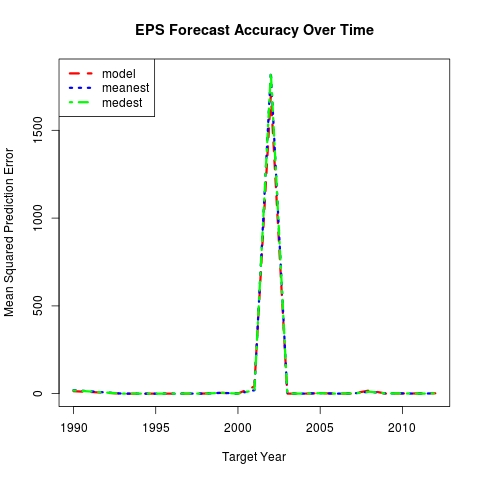
\includegraphics[height=4in]{../graphics/eps-by-year-fy1.jpeg}
%    \caption{Mean squared prediction error for model and consensus forecasts by target forecast year.}
%    \label{spe-by-year-graph-fy1}
%  \end{center}
%  \end{figure}
  
\textbf{Does private information help analyst forecasts?} Table \ref{evaluation-regfd} presents
comparisons of the model's accuracy before and after implementation of Regulation Fair Disclosure. 
As noted in prior literature (e.g. \cite{gintschelmarkov2004}) analyst forecasts are worse in the 
post-Reg FD period. The performance of the model forecasts does not change in any consistent way
pre- and post-Reg FD.\footnote{In this section and all others, ``consensus'' forecasts refer to the
mean analyst estimate. Results with median analyst estimates are qualitatively similar.}


\textbf{The effects of \emph{ex ante} uncertainty on forecasts.} Table \ref{evaluation-dispersion}
presents comparisons of the accuracy of model and consensus forecasts during information 
environments characterized by high and low uncertainty. Both the model and analyst forecasts 
perform better during periods characterized by low analyst dispersion.\footnote{Dispersion is 
measured as the standard deviation of analyst forecasts. High (low) dispersion periods are those
with a standard deviation above (below) the median. Results are not sensitive to choice of 
percentile.} For the one-year-ahead forecasts, the model performs relatively better than consensus
forecasts.

%\subsection{Implied Cost of Capital}

%\subsection{Market Equity Premium}

\subsection{Earnings Forecasts as Trading Signals}
Most studies that compare time series forecasts to analyst forecasts use a loss function (evaluation
criterion) that is some form of relative prediction error or bias. To better quantify the 
significance of divergence between the consensus forecasts of earnings and the model forecast, I 
examine the returns
to an investor who uses the divergence in analyst and model forecasts as a signal. As a first step,
I calculate buy and hold returns ($BAHR$) for each firm from the forecast date to one month and, 
separately,
two months after the target date (i.e., the date at which forecasted earnings are revealed.) I do 
this for all forecasts (one-, two-, and three-year-ahead forecasts.) I then compute the divergence
between the model forecasts and the consensus forecast, $DIFF$, as the model forecast less the 
consensus forecast. $DIFF$ is calculated for each forecast horizon. For each forecast target and 
returns horizon I run a regression of the form

\begin{equation}
BAHR_{t+\tau} = \alpha_{0} + \alpha_{1}DIFF_{i} + \varepsilon.
\end{equation}

Table \ref{evaluation-bahr} shows the coefficient and p-values from each of these regressions. 
For the forecasts of FY1 earnings, buy-and-hold returns are positively and statistically 
significantly related to the degree of 
divergence between model forecasts and consensus analyst forecasts. Note, however, that
returns have not been adjusted for standard asset pricign risk factors.
\\

Next, I rank and group each forecast into deciles by the level of divergence. As Figures
\ref{bahr-diff-decile} and \ref{bahr-diff-decile2} show, the buy-and-hold returns over the forecast
horizon for the forecast of FY1 earnings is increasing in the level of divergence between the model
and the consensus forecast. This indicates that the stock returns of firms for which the model
forecasts higher earnings than analysts are higher than those for which analysts are more optimistic
than the model suggests.
\\

  
\section{Conclusions and Extensions}
Research that relies on analyst forecasts of earnings suffers from three flaws: (1) analyst 
forecasts are known to be upwardly biased; (2) there is evidence suggesting analysts don't
attempt to accurately forecast earnings and investors don't necessarily rely on these forecasts
explicitly for information about long-term cash flows; and (3) since the availability of machine-
readable analyst forecasts only dates back to the early 1980s, the research sample is necessarily
limited. The statistical forecasts of earnings from firm-level regressions that I develop here
overcomes the first and last points. By demonstrating that the forecasts from my model are 
associated with higher returns I provide support for the notion that some market participants
may be able to derive more accurate from the past history of earnings than is given by blindly
following analyst forecasts. To fully address the second point, the forecasts from my model must
be used to derive implied cost of capital estimates and market risk premia. If the forecasts
represent a better proxy for market-level expectations then they may lead to estimates that
better conform to the risk-return relationship predicted by modern asset pricing theory. I leave 
this step for future work.

\bibliographystyle{aea}
\bibliography{articles}
\newpage
\section*{Appendix: Tables and Figures}
% latex table generated in R 3.0.2 by xtable 1.7-3 package
% Tue Aug 26 15:23:31 2014
\begin{table}[H]
\centering
\begin{tabular}{lrrrrr}
  \hline
 & mean & med & min & max & stdev \\ 
  \hline
EPS & 1.504 & 1.165 & -21.690 & 89.610 & 2.103 \\ 
  EPS Growth & 0.126 & 0.121 & -246.500 & 768.000 & 8.127 \\ 
  Total Assets & 8858.471 & 2038.377 & 48.195 & 797769.000 & 30477.603 \\ 
  Accruals & -0.030 & -0.037 & -1.013 & 2.832 & 0.121 \\ 
  Dividends & 0.541 & 0.274 & 0.000 & 51.403 & 0.929 \\ 
  Dividend Payer & 0.203 & 0.000 & 0.000 & 1.000 & 0.402 \\ 
  Negative Earnings & 0.056 & 0.000 & 0.000 & 1.000 & 0.229 \\ 
  Delta Price & 0.083 & 0.038 & -2.674 & 14.366 & 0.486 \\ 
  return & -0.003 & 0.038 & -3.501 & 2.732 & 0.422 \\ 
  PE Ratio & 59.508 & 24.157 & -110000.000 & 151250.000 & 1635.234 \\ 
  GDP & 0.048 & 0.049 & -0.032 & 0.124 & 0.023 \\ 
  ROE & 0.482 & 0.147 & -282.640 & 5822.013 & 44.669 \\ 
  Unemployment & 0.062 & 0.056 & 0.038 & 0.108 & 0.017 \\ 
  Inflation (PPI) & 0.003 & 0.003 & -0.053 & 0.030 & 0.011 \\ 
  Sales & 8096.594 & 1975.248 & -7.237 & 470171.000 & 25083.807 \\ 
  AR & 1497.423 & 258.700 & 0.000 & 418777.000 & 10231.124 \\ 
  AP & 783.347 & 127.400 & 0.000 & 149813.000 & 3446.179 \\ 
  Age & 16.396 & 15.000 & 5.000 & 32.000 & 7.977 \\ 
 $\Delta Sales$ & 832.864 & 154.138 & -295570.000 & 368056.000 & 7283.693 \\ 
  $\Delta AR$ & 128.839 & 18.461 & -45714.199 & 99095.000 & 1780.134 \\ 
  $\Delta AP$ & 76.889 & 8.921 & -83588.000 & 71555.000 & 1149.442 \\ 
   \hline
\end{tabular}
\captionsetup{width=4in, font=footnotesize}
\caption{Summary statistics of EPS and independent variables. $Age$ is number of years company is in the sample.}
\label{summary-stats}
\end{table}

% latex table generated in R 3.1.1 by xtable 1.7-4 package
% Thu Feb 26 16:52:22 2015
\begin{table}[ht]
\centering
\begin{tabular}{rrrrrr}
  \hline
 & mean & med & min & max & stdev \\ 
  \hline
$EPS_{t-1}$ & 0.8027 & 0.8753 & -0.1915 & 1.6592 & 0.2938 \\ 
assets & 0.0408 & 0.0211 & -0.2675 & 1.2235 & 0.1008 \\ 
  Accruals & 1.1515 & 0.1889 & -27.7192 & 51.6659 & 5.7370 \\ 
  Dividends & -1.9528 & -0.0001 & -868.1679 & 101.1100 & 44.6254 \\ 
  Negative Earnings & 0.2092 & 0.1332 & -4.6542 & 5.7750 & 1.4040 \\ 
  $\Delta Price$ & 0.5412 & 0.2741 & -1.0112 & 29.5364 & 1.5372 \\ 
  return & 0.5667 & 0.2829 & -1.0074 & 31.0738 & 1.6127 \\ 
  PE Ratio & -0.0036 & -0.0004 & -0.2647 & 0.0760 & 0.0213 \\ 
  GDP & 3.4401 & 1.8823 & -122.6991 & 64.2745 & 12.9067 \\ 
  ROE & 2.0801 & 0.9929 & -6.2682 & 24.3831 & 3.4486 \\ 
  Unemployment & -1.2504 & 0.1596 & -176.6090 & 97.6023 & 21.2597 \\ 
  Inflation (PPI) & 10.6295 & 4.8897 & -162.8660 & 168.6141 & 27.7419 \\ 
  Sales & 0.5747 & 0.3485 & -3.3250 & 9.0993 & 1.1306 \\ 
  AR & 0.0681 & 0.0322 & -0.3495 & 1.7380 & 0.1476 \\ 
  AP & 0.0757 & 0.0435 & -0.3640 & 1.6566 & 0.1532 \\ 
  $\Delta Sales$ & 0.0004 & 0.0001 & -0.0022 & 0.0093 & 0.0009 \\ 
  $\Delta AR$ & 0.0018 & 0.0005 & -0.0268 & 0.1659 & 0.0091 \\ 
  $\Delta AP$ & 0.0023 & 0.0008 & -0.0631 & 0.0523 & 0.0086 \\ 
   \hline
\end{tabular}
\caption{Coefficients from regressions of the form $EPS_{t} = \alpha_0 + \alpha_{1}EPS_{t} + \alpha_{2}X_{t-1} +\varepsilon.$} 
\label{univariate-stats-eps-rsquared}
\end{table}
% latex table generated in R 3.0.2 by xtable 1.7-3 package
% Thu Aug 28 12:40:48 2014
\begin{table}[H]
\centering
\begin{tabular}{rrrrrr}
  \hline
 & mean & med & min & max & stdev \\ 
  \hline
$EPS_{t-1}$ & 0.6226 & 0.6972 & 0.0002 & 0.9981 & 0.3130 \\ 
assets & 0.6440 & 0.7110 & 0.0013 & 0.9982 & 0.2984 \\ 
  Accruals & 0.6491 & 0.7069 & 0.0068 & 0.9983 & 0.2849 \\ 
  Dividends & 0.6490 & 0.7168 & 0.0063 & 0.9984 & 0.2962 \\ 
  Negative Earnings & 0.6353 & 0.7079 & 0.0006 & 0.9981 & 0.2995 \\ 
  $\Delta Price$ & 0.6901 & 0.7469 & 0.0224 & 0.9981 & 0.2624 \\ 
  return & 0.6957 & 0.7549 & 0.0179 & 0.9981 & 0.2588 \\ 
  PE Ratio & 0.6431 & 0.7152 & 0.0128 & 0.9982 & 0.2961 \\ 
  GDP & 0.6578 & 0.7366 & 0.0062 & 0.9983 & 0.2927 \\ 
  ROE & 0.7294 & 0.7957 & 0.0045 & 0.9982 & 0.2406 \\ 
  Unemployment & 0.6618 & 0.7358 & 0.0010 & 0.9984 & 0.2877 \\ 
  Inflation (PPI) & 0.6647 & 0.7364 & 0.0296 & 0.9982 & 0.2829 \\ 
  Sales & 0.6870 & 0.7596 & 0.0009 & 0.9982 & 0.2743 \\ 
  AR & 0.6497 & 0.7148 & 0.0010 & 0.9983 & 0.2931 \\ 
  AP & 0.6514 & 0.7234 & 0.0079 & 0.9982 & 0.2932 \\ 
$\Delta Sales$ & 0.7089 & 0.7838 & 0.0047 & 0.9984 & 0.2684 \\ 
$\Delta AR$ & 0.6744 & 0.7403 & 0.0110 & 0.9983 & 0.2781 \\ 
$\Delta AP$ & 0.6690 & 0.7364 & 0.0027 & 0.9981 & 0.2822 \\ 
   \hline
\end{tabular}
\captionsetup{width=4in, font=footnotesize}
\caption{$R^2$ values from regressions of the form $EPS_{t} = \alpha_0 + \alpha_{1}EPS_{t} + \alpha_{2}X_{t-1} +\varepsilon.$} 
\label{univariate-stats-eps-rsquared}
\end{table}
% latex table generated in R 3.0.2 by xtable 1.7-3 package
% Sun Aug 31 11:31:11 2014
\begin{table}[H]
\centering
\begin{tabular}{rrrr}
  \hline
Year & Model & MEANEST & MEDEST \\ 
  \hline
1990 & 14.440 & 20.250 & 18.662 \\ 
1993 & 0.116 & 0.152 & 0.176 \\ 
1994 & 0.096 & 0.137 & 0.137 \\ 
1995 & 0.166 & 0.037 & 0.031 \\ 
1996 & 0.122 & 0.002 & 0.000 \\ 
1997 & 0.180 & 0.554 & 0.606 \\ 
1998 & 1.018 & 0.196 & 0.201 \\ 
1999 & 4.547 & 5.233 & 5.126 \\ 
2000 & 0.542 & 0.379 & 0.324 \\ 
2001 & 41.042 & 19.687 & 19.687 \\ 
2002 & 1701.955 & 1832.864 & 1828.333 \\ 
2003 & 0.152 & 0.151 & 0.148 \\ 
2004 & 0.263 & 0.365 & 0.359 \\ 
2005 & 2.929 & 2.737 & 2.749 \\ 
2006 & 0.593 & 0.211 & 0.209 \\ 
2007 & 0.771 & 1.316 & 1.389 \\ 
2008 & 18.404 & 11.094 & 11.298 \\ 
2009 & 0.592 & 1.357 & 1.303 \\ 
2010 & 1.658 & 1.379 & 1.381 \\ 
2011 & 1.016 & 0.367 & 0.378 \\ 
2012 & 2.357 & 1.612 & 1.618 \\ 
   \hline
\end{tabular}
\captionsetup{width=3in, font=footnotesize}
\caption{Mean squared prediction error of model forecast, mean analyst (MEANEST) forecast, and 
median analyst forecast (MEDEST). Forecasts are of one-year-ahead earnings.} 
\label{spe-by-year-table-fy1}
\end{table}

\begin{table}[H]
\centering
\begin{tabular}{l | c c | c c}
  \hline
&  \multicolumn{2}{| c}{Pre-Reg FD} &  \multicolumn{2}{| c}{Post-Reg FD} \\
% & Pre-Reg FD & & Post-Reg FD & \\ 
  \hline
 Forecast horizon & Model & Consensus & Model & Consensus \\ 
  \hline
1-Year Ahead & 2.365 & 2.466 & 27.479 &28.159 \\ 
2-Year Ahead & 2.255 & 1.905 & 4.163 & 3.672 \\ 
3-Year Ahead & 0.732 & 2.574 & 3.889 & 4.256 \\ 
   \hline
\end{tabular}
\captionsetup{width=4in, font=footnotesize}
\caption{Mean squared prediction error comparison of ``model'' and ``consensus'' earnings forecasts.}
\label{evaluation-regfd}
\end{table}

\begin{table}[H]
\centering
\begin{tabular}{l | c c | c c}
  \hline
&  \multicolumn{2}{| c}{Low Dispersion} &  \multicolumn{2}{| c}{High Dispersion} \\
  \hline
 Forecast horizon & Model & Consensus & Model & Consensus \\ 
  \hline
1-Year Ahead & 1.45 & 0.774 &90.436 & 94.511 \\ 
2-Year Ahead & 8.133 & 7.853 & 0.874 & 0.371 \\ 
3-Year Ahead & 1.409 & 0.860 & 5.155 & 4.986  \\ 
   \hline
\end{tabular}
\captionsetup{width=4in, font=footnotesize}
\caption{Mean squared prediction error comparison of ``model'' and ``consensus'' earnings forecasts.}
\label{evaluation-dispersion}
\end{table}

\begin{table}[H]
\centering
\begin{tabular}{l | c c | c c}
  \hline
&  \multicolumn{2}{| c}{BAHR $\tau+1$ month} &  \multicolumn{2}{| c}{BAHR $\tau+2$ months}  \\
  \hline
 Forecast horizon, $\tau$ & Coeff. & \emph{P-Value} &  Coeff. & \emph{P-Value}  \\ 
  \hline
1-Year Ahead & 0.06825** & 0.0334 & 0.06903** & 0.0329 \\ 
%1-Year Ahead & 1.706 & 1.230 & -11.060 & 38.150 \\ 
2-Year Ahead & 0.02169 & 0.344 & 0.02610 & 0.259 \\ 
%2-Year Ahead & 1.706 & 1.230 & -11.060 & 38.150 \\ 
3-Year Ahead & -0.02812 & 0.216 & -0.02903 & 0.205 \\ 
%3-Year Ahead & 1.706 & 1.230 & -11.060 & 38.150 \\ 
   \hline
\end{tabular}
\captionsetup{width=4in, font=footnotesize}
\caption{Buy-and-hold returns for FY1 ($\tau=12$), FY2 ($\tau=24$), and FY3 ($\tau=36$) 
forecasts. Return horizons are one month and two months after the forecast target date.}
\label{evaluation-bahr}
\end{table}


  \begin{figure}[H]
  \begin{center}
    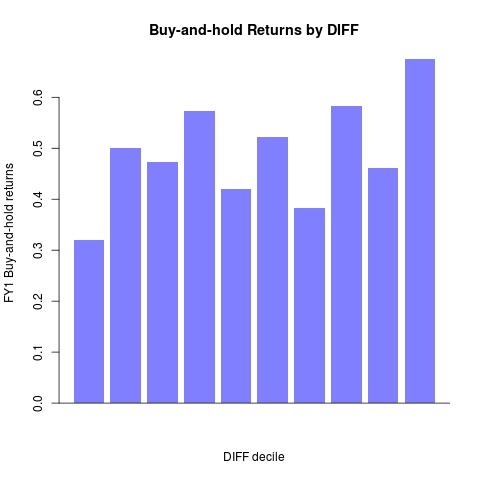
\includegraphics[height=4in]{../graphics/bahr-diff-decile.jpeg}
    \captionsetup{width=4in, font=footnotesize}
    \caption{Buy-and-hold returns by $DIFF$ decile for one-year-ahead model. $DIFF$ is the model 
    forecast of earnings less the consensus forecast.}
    \label{bahr-diff-decile}
  \end{center}
  \end{figure}

  \begin{figure}[H]
  \begin{center}
    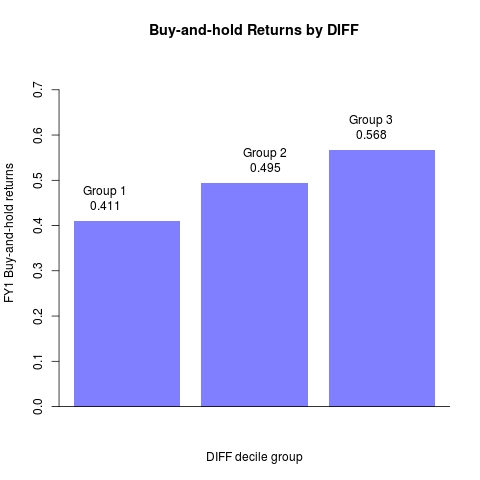
\includegraphics[height=4in]{../graphics/bahr-diff-decile2.jpeg}
    \captionsetup{width=4in, font=footnotesize}
    \caption{Buy-and-hold returns by $DIFF$ decile for one-year-ahead model. $DIFF$ is the model 
    forecast of earnings less the consensus forecast. Group 1: first and second decile. Group 3: 
    ninth and 10th deciles.}
    \label{bahr-diff-decile2}
  \end{center}
  \end{figure}
\end{document}
